\documentclass[M3_Night4_Solutions]{subfiles}

\IfSubStr{\jobname}{\detokenize{Solutions}}{\toggletrue{solutions}}{\togglefalse{solutions}}

\fancypagestyle{firstpage}

{\rhead{Night 4 \linebreak \textit{Version: \today}}}

\title{Night 4: Optimization and Gradient Ascent}
\author{Quantitative Engineering Analysis}
\date{Spring 2019}

\begin{document}

\maketitle
\thispagestyle{firstpage}

\section{Learning Goals}
By the end of this assignment, you should feel confident with the following:
\bi
\item Extending the idea of optimization
\item Partial derivatives and the gradient
\item Unconstrained optimization: concept and the method of steepest ascent
\ei

\section{Conceptual Exercise: The Leisure Seeker [1 Hr]}

The map below gives the temperature across the United States on a certain winter day.  
Regions of the same color have the same temperature: violet 
represents the coldest areas, and temperatures rise as the colors traverse the 
spectrum from indigo to blue to green to yellow to orange to red.
\begin{center}

\includegraphics[width=5in]{figs/WeatherMap.pdf} 
\end{center}

Locate Chicago on the map and mark it with a dot.  The weather in Chicago is 
freezing in winter, so a resident of the city decides to embark on a journey in 
search of the sun.  From Chicago,  she wants to travel in the direction in which 
temperature rises most quickly.  

\be[series=exercises, label=\textbf{Exercise} (\arabic*)]
\item In which direction should she go? Draw an arrow, starting at Chicago, that indicates this direction. 
\ee 

As her journey proceeds,  she decides to keep traveling in the direction in which the 
weather warms up most quickly: wherever she is at any moment, she moves in the 
direction of fastest temperature rise.  

\be[resume=exercises, label=\textbf{Exercise} (\arabic*)]
\item Make a rough sketch of the route she takes.  
\solution{See Fig.\ \ref{posspath}.
\begin{center}
\label{posspath}
\includegraphics[width=5in]{figs/paths.png} 
\end{center}
}
\item Where does she end up, assuming that she doesn't leave the United States?  
\solution{Near Panama City, FL}
\item What would happen if her friend started in Billings, Montana?  Where would he end up? 
\solution{Hard to know exactly without more isotherms (contours of constant temperature), but maybe the SF Bay Area or the Portland area.}


\ee

\section{Readings, Videos, and Conceptual Questions - Partials and Gradients [3 Hrs]}

At this \href{https://sites.google.com/site/linearity2fall2014/partial-derivative-videos}{link} you will find a set of readings and videos about partial derivatives, the gradient, and the Hessian.  Some of this is stuff you already dealt with in the boats and faces modules; some of it is new.
Read the text and/or watch these videos, and then write short qualitative answers to the following questions: 
%I feel like my solutions to these conceptual questions could use some revision next year -ET

\be[resume=exercises, label=\textbf{Exercise} (\arabic*)]
\item What is meant by $f_x$?  By $\frac{\partial^2 f}{\partial x^2}$?  By $D_u f$?  By $\nabla f$? 
\solution{The partial derivative with respect to $x$, meaning the slope in the $x$ direction (where every other independent variable is held constant); the second partial derivative with respect to $x$, meaning the curvature in the $x$ direction (where every other independent variable is held constant); the directional derivative with respect to vector $u$, meaning the slope in the $u$ direction; the gradient, meaning the maximum slope in its corresponding direction.}
\item In Stewart, the idea of gradient is discussed primarily in two dimensional and three dimensional ``physical'' spaces, using $\ihat$, $\jhat$, and so forth.  But more generally, you can have a gradient of a function of any number of variables.  Give a real-world example of a gradient for a situation that involves more than 3 variables.
\solution{Any kind of optimization problem could have a gradient of the objective function in many dimensions (decision variables).}
\item ``The gradient always points in the direction of fastest increase.''  Can you think of physical examples where there is {\it more than one} direction of fastest increase?  What's going on here?
\solution{At the bottom of a cone, the increase is equally fast in all directions.}
\item ``The gradient is always normal to level curves/surfaces.''  Explain.
\solution{A differential surface area at any given point on a surface is flat, an can be defined by the line where it intersects with the level curve and a perpendicular line in the direction of greatest increase. Therefore, the gradient if normal to a level curve.}
\item ``The directional derivative in the direction of $\u$ is given by $\nabla f \cdot \hat{\u}$.''  Why does this make sense?
\solution{The gradient could be decomposed into a component in $\hat{\u}$  direction and a component normal to that. So the rate of change of the function in the $\hat{\u}$  direction is $\nabla f \cdot \hat{\u}$.}
\item If the gradient is zero, does that imply that you are at a max or a min?  Why or why not?
\solution{No, because you could be at a saddle point, for example.}
\item What does it mean for $\frac{\partial^2 f}{\partial x^2} >0$?  What about   $\frac{\partial^2 f}{\partial x \partial y} >0$?
\solution{Upward curvature in the x-direction; slope in x-direction increases with increasing y (and vice versa).}
\ee

\be[resume=exercises, label=\textbf{Exercise} (\arabic*)]

\item The diagram below shows a contour plot for a function. Sketch in the gradient field.

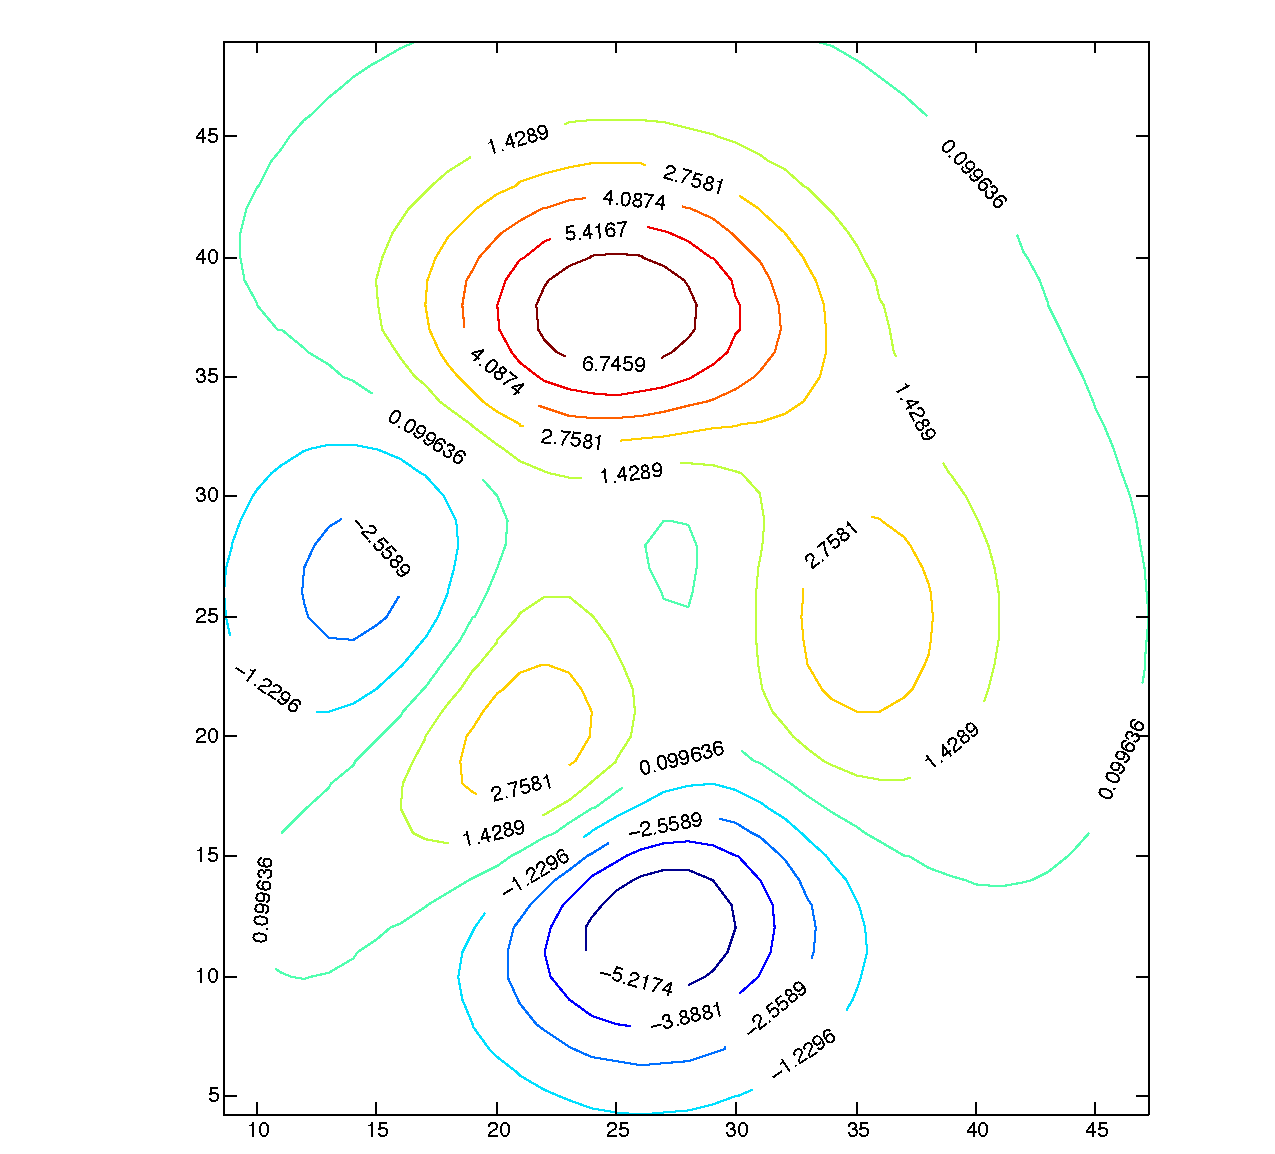
\includegraphics[width=4in]{figs/LabeledContourPlot.pdf}
\solution{\includegraphics[width=4in]{figs/sol1.png}}

\item The diagrams below show two vector fields.  One is the gradient of a function of two variables; the other is not.  Which one could be a gradient?  Why?  Sketch in the level curves for the one that works.

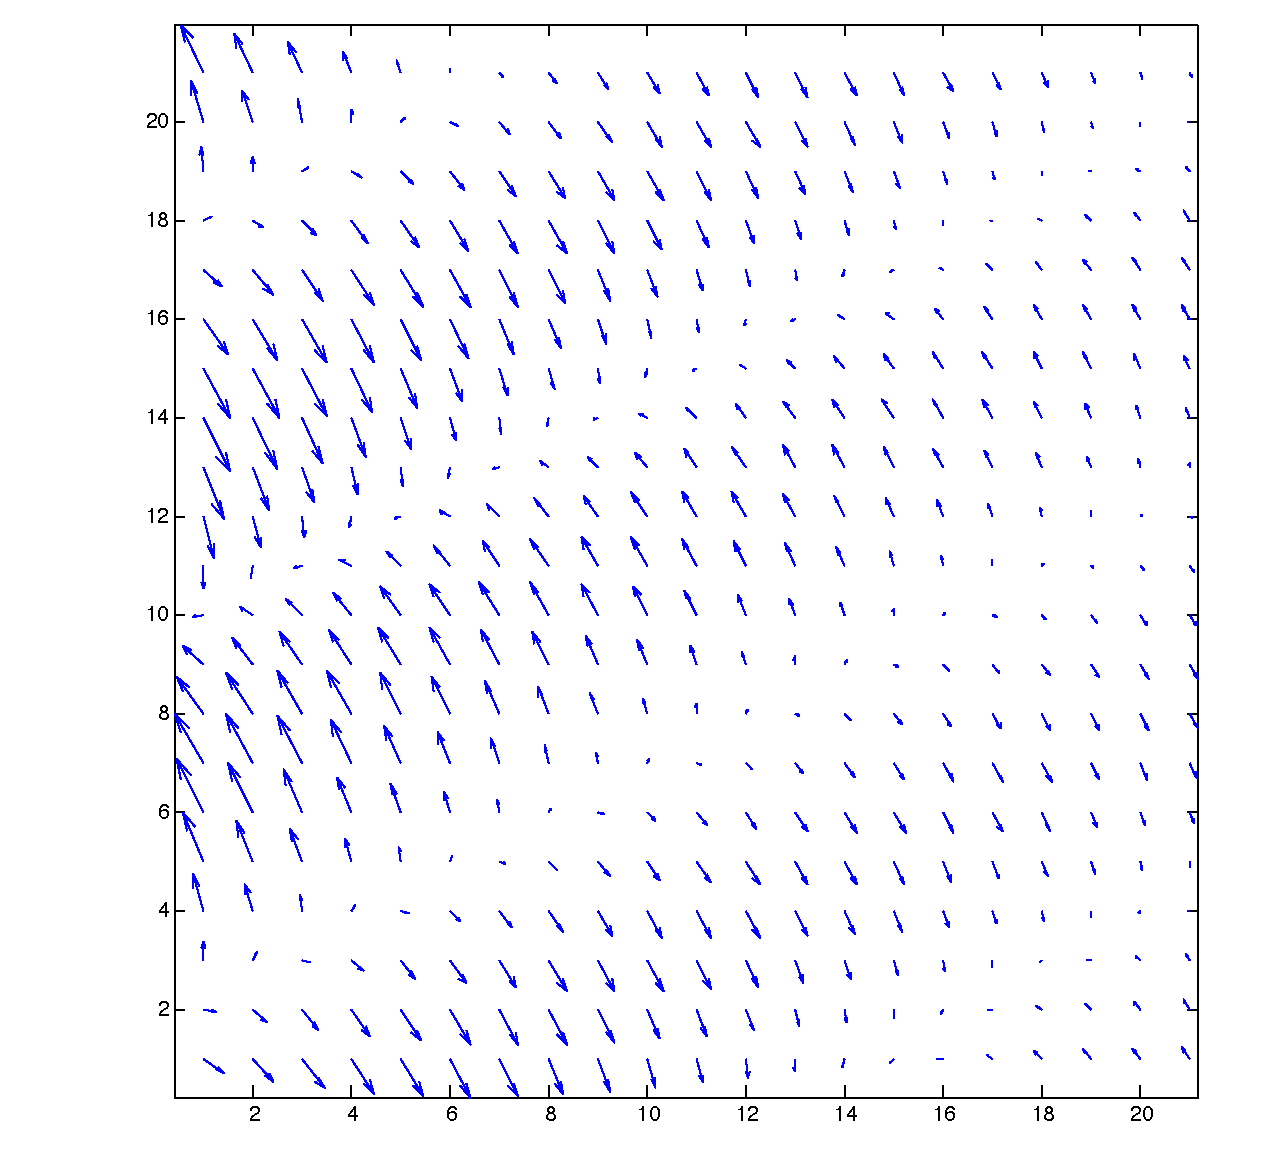
\includegraphics[width=3in]{figs/ConservativeQuiver.pdf}
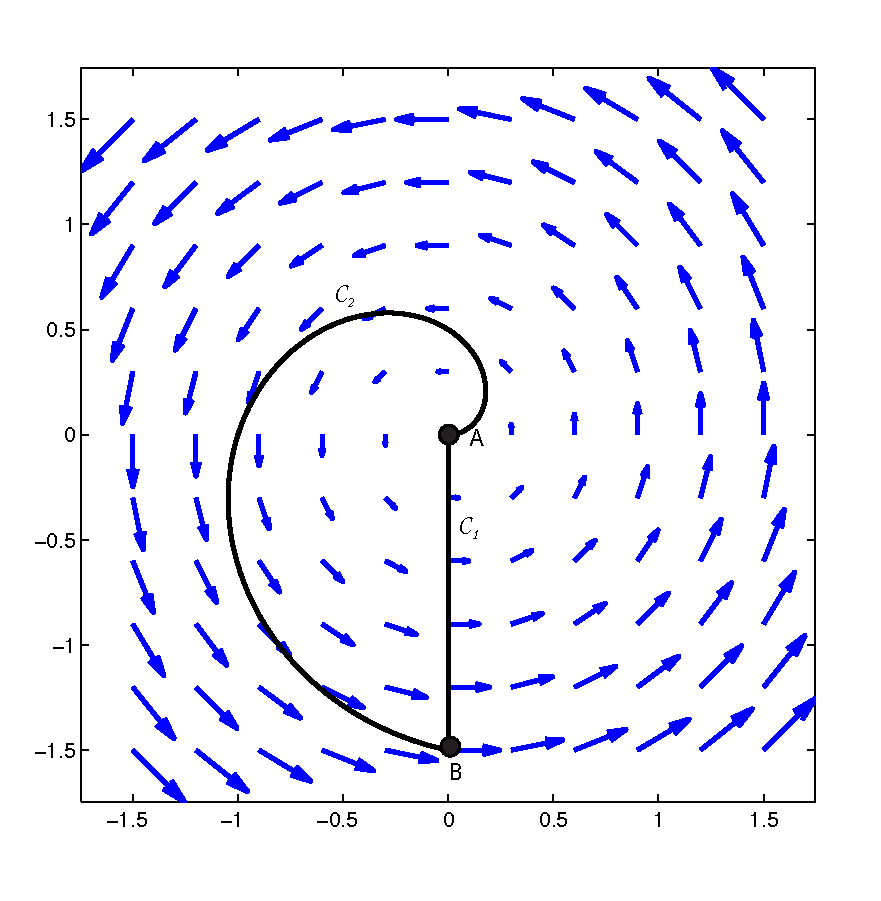
\includegraphics[width=3in]{figs/CirculationQuiver.pdf}

\solution{The one on the left could be a gradient; the left one could not because a path of gradient ascent would go in a circle. See FIg.\ \ref{sol22} for a sketchy sketch of level curves.
\begin{center}
\label{sol22}
\includegraphics[width=3in]{figs/sol2.png} 
\end{center}
}

\item A function $f$ has the graph shown below.  The grid lines on the graph are lines 
along which either the $x$- or the $y$- coordinate is held constant.

\includegraphics[width=6in]{figs/Graph_ContourLines} 

Determine the sign of each of the following:
\begin{multicols}{2}
\begin{enumerate}
\item $f_x(1, 2)$
\item $f_y(1, 2)$
\item $f_{xx}(1, 2)$
\item $f_{yy}(1, 2)$
\end{enumerate}
\end{multicols}
\solution{(a)+; (b) +; (c) and (d) look pretty close to 0.}

\item The diagram below shows some level curves of a function $g(x,y)$.  The numbers 
indicate the $g$-values of these level curves, and the letters indicate points on the level curves.  Note that point $Y$ is on  the level curve $g = 1$ and point $W$ is on the level curve $g = -2$.

\includegraphics[width=5in]{figs/LevelCurves} 

\be
\item
What are the signs of the partial derivatives $\frac{\partial g}{\partial x}$ and 
$\frac{\partial g}{\partial y}$at each of the points marked? Why?
\solution{
\begin{table}[h!]
\begin{tabular}{ccc}
Point  & Sign of $g_x$ & Sign of $g_y$ \\
R & - or 0     & +          \\
S & -          & +          \\
T & -          & 0          \\
U & 0          & -          \\
V & +          & 0          \\
W & -          & -          \\
X & 0          & -          \\
Y & +          & +         
\end{tabular}
\end{table}}

\item
At which of the points marked does the gradient 
vector $\nabla g$ have the greatest magnitude?  Explain.
\solution{At Y because the contours are closest together, indicating the greatest change in the function value per unit distance normal to the level curves.}
\item
Let  
\[ \u = \begin{bmatrix} 1 \\ 1 \end{bmatrix}.\]
The directional derivative $D_{\hat{\u}} g$ is zero at exactly one of the points marked.  Which point is it?
\solution{Point S, where the contour line is parallel to $\u$.}

\ee

\ee




\section{Readings, Videos, and Conceptual Questions - Optimization with  Gradient Ascent [2 Hrs]}
At this  \href{https://sites.google.com/site/linearity2fall2014/partial-derivative-videos}{link}  you will {\it also} find a set of readings and videos about gradient ascent (or descent - same thing, but for a sign!). 

Read the text from Giordano and watch the videos.  If you are interested, you can also read the stuff about conjugate gradient ascent, which is cool and leverages eigenstuff - but is optional! 

Then answer the following questions: 

\begin{enumerate}[resume=exercises, label=\textbf{Exercise} (\arabic*)]
%\item There is a mistake in the Part 4 of the Hessian video.  Find it. \todo{I don't like these sorts of questions. What are trying to have them notice here?}
\item At the origin, a given function has a gradient of $\twobyone{1}{1}$ and a Hessian of 
\[ \twobytwo{2}{3}{3}{4} \]
Sketch a contour plot of the function in the vicinity of the origin.
\solution{One example would be $x^2+2y^2+x+y+3xy$:

\includegraphics[width=3in]{figs/ans} 

Important features are:
\be
\item Level curves get closer together as x and y increase (near the origin)
\item Level curve at the origin is in direction $\twobyone{1}{-1}$
\item Level curves near the origin tip upward (become more horizontal) as x and y increase
\ee}

\clearpage
\item The figure below shows a contour plot with two points marked (A and B).  For both points, 

\be
\item Draw the path that gradient ascent would use if the step size was small (following the approach in the first video).
\item Draw the path that gradient ascent would follow if the algorithm is implemented as shown in the second video. 


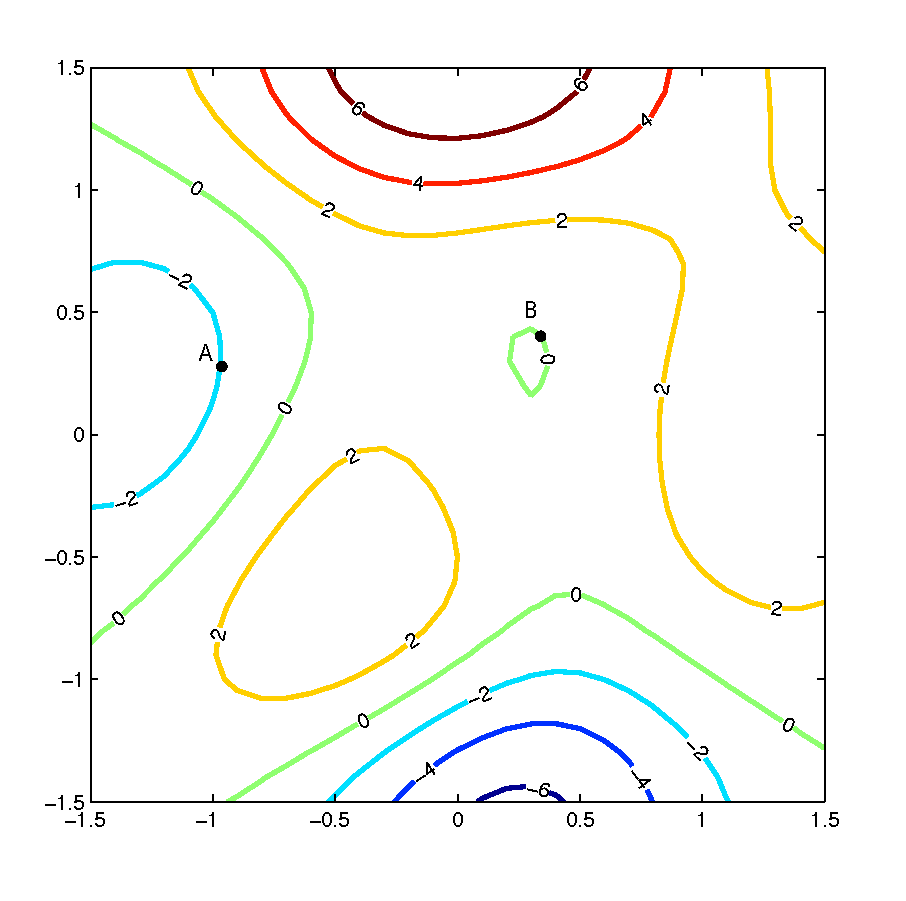
\includegraphics[width=6in]{figs/ContourExample3.pdf} 
\solution{\includegraphics[width=3in]{figs/fourpaths.png} 

The black path is the small step size ascent; the purple and blue paths are the walk-straight-until-you-start-to-go-downhill method. But it's a little hard to predict the path from point A given the large spacing of contours...other reasonable paths will be accepted.}

\ee

\clearpage

\ee

%\section{Gradient Ascent in Code [1 Hr]}
%
%\begin{enumerate}[resume=exercises, label=\textbf{Exercise} (\arabic*)]
%\item In MATLAB...
%\be
%\item Implement the steepest ascent method described by Giordano using the multiplier technique of $\lambda_{k+1} = \delta \lambda_{k}$.  
%\item Using your code, numerically find a local maximum of $$f(x,y) = xy - x^2 -y^2 -2x-2y +4$$  Start your search at the point $x=4, y=0$, and produce a plot that shows the first 10 moves toward the maximum.
%\item Verify your numerical answer by evaluating the Hessian and the gradient.
%\ee
%\ee


\section{Gradient Ascent [2 Hrs]}
As you've just been learning, Gradient Ascent (or descent) is a technique to determine the maximum or minimum of a function of many variables by taking steps in the direction of the gradient (or negative gradient). If the height of a surface is described by $z = f(\r)$, where $\r$ is the position vector in the plane, and we begin at $\r_0$, the points determined by Gradient Ascent are given by
\[\r_{i+1} = \r_{i} + \lambda_{i} \nabla f(\r_i), \; i = 0,1,2, \ldots \]
where $\lambda_{i}$ is the relative size of the step that we take in the direction of the gradient. There are various schemes for choosing these, and one of the simplest is to determine the next step with a simple proportionality
\[\lambda_{i+1} = \delta \lambda_{i} \]
where both $\delta$ and $\lambda_0$ are thoughtfully chosen for the problem at hand. We are going to develop a method and implementation to drive your NEATO on the floor of the classroom in a way that physically realizes the method of Steepest Ascent. First, we are going to introduce the mountain you will climb, and you will think through the steps involved.

\be[resume]
\item  The mountain you will "climb" is defined as follows
\[ f(x,y) = xy - x^2 - y^2 -2x -2y + 4 \]
where $x$, $y$, and $f$ are measured in feet. You are required to start at $(1,-1)$, and work your way to the top by method of steepest ascent.
\be
\item Visualize the contours of this function in MATHEMATICA on the domain $(-3,1) \times (-3,1)$, and print it out. 
\solution{\includegraphics[width=3in]{figs/oval.png} }
\item Draw the path of steepest ascent if we were moving continuously from a starting point at $(1,-1)$.  
\item Find the gradient of this function.
\solution{$(-2 - 2 x + y, -2 + x - 2 y)$}
\item Assuming $\r_0 = (1,-1)$, what is the initial gradient at $\r_0$? What would be a reasonable choice for $\lambda_0$ so that $\r_1$ is not too far from the continuous path? Plot $\r_1$ on your contour plot.
\solution{Initial gradient is (-5,1), with a magnitude of 5.1. To move about 0.5 feet, the initial multiplier $\lambda_0$ should be about 0.1 feet. }
\item Assuming you place your NEATO at $(1,-1)$ pointing along the y-axis, how much do you have to rotate it in order to align it with the gradient at $\r_0$? What would be a reasonable angular speed?
\solution{1.37 rad (78.7 degrees) CCW. 0.5 rad/s would not exceed 0.3 m/s if rotated in place.}
\item Assuming that you are going to drive your NEATO at $0.1 m/s$, how long would you drive in order to reach $\r_1$? (Careful with unit changes!)
\solution{$t=\frac{|\r_1-\r_0|}{V} \frac{1 {\rm m}}{3.28 {\rm ft}}$}
\item What is the gradient at $\r_1$? What value of $\delta$ should you use so that $\lambda_1$ and $\r_2$ are reasonable? Plot $\r_2$ on your contour plot.
\item Assuming your NEATO is now at $\r_1$, how much do you have to rotate it in order to align it with the new gradient? What would be a reasonable angular speed?
\item Assuming that you are going to drive your NEATO at $0.1 m/s$, how long would you drive in order to reach $\r_2$?
\ee
\ee

%%{\bf Paul and Rebecca: I chose this so that it looks good over the domain of (-3,1)x(-3,1). The maximum is at $(-2,2)$, and if you start at (1,0) you generally take a curving path to the top.}
%\vspace{1em}
%\textbf{Note:} for your first time working through this problem you should do everything based purely on timing (as we did in the Bridge of Death).  For instance, if you calculate that you should rotate your robot by an angle $\theta$ you should execute the following steps: choose an angular velocity $\omega$ (it is up to you how fast you want to rotate, but slower rotations will generally be more accurate), calculate the appropriate wheel velocities, send these velocities to the robot, and stop the robot after $\frac{\theta}{\omega}$ seconds (the \emph{pause} command may be useful).
%
%\be
%\item Review the work you did on finding the maximum of this function using the method of Steepest Ascent. Edit the method that you used in order to start at $\r_0=(4,0)$. What is the initial gradient at $\r_0$? What is $\r_1$? What is the distance between $\r_0$ and $\r_1$? What is the gradient at $\r_1$? What is $\r_2$? What is the distance between $\r_1$ and $\r_2$?
%\item Assuming you place your NEATO on the floor at $(4,0)$ and align it so that it is pointing in the $y$-direction, how do you rotate it so that it points in the direction of the initial gradient?
%\item Assuming that you are going to drive it at $0.1 m/s$, how long do you drive for in order to reach $\r_1$?
%\item You will need to think about rotating and moving at every step. Don't forget that you will need to keep track of your NEATO heading!
%\ee
%\ee
%
%\section{Optional Extension}
%If you managed the previous exercise, how about if we determine the continuous path of steepest ascent, and drive your NEATO along this path using the techniques from the bridge of death? Sounds like fun, right!
%
%If we want to follow the continuous path of steepest ascent, we should set the velocity of the NEATO proportional to the gradient, $\r'(t) = \alpha \nabla f$, where $\alpha$ is a parameter that we can choose depending on how fast we want the NEATO to drive.
%
%\be[resume]
%\item How does the speed of the NEATO depend on $\alpha$ and $\nabla f$? If $\alpha$ is a constant, how fast is the NEATO moving when it reaches the "top" of the hill? How would we choose $\alpha$ if we wanted the NEATO to move with constant forward velocity $v$?
%\item In terms of coordinates $x$ and $y$ this approach is equivalent to defining the following set of ordinary differential equations, of the type that you encountered in ModSim
%\begin{eqnarray*}
%\frac{dx}{dt} &=& \alpha \frac{\partial f}{\partial x} \\
%\frac{dy}{dt} &=& \alpha \frac{\partial f}{\partial y}
%\end{eqnarray*}
%where $x(0)$ and $y(0)$ represent the initial position of the NEATO. You can either solve these in MATHEMATICA using DSolve, in MATLAB using dsolve (\href{https://www.mathworks.com/help/symbolic/solve-a-single-differential-equation.html}{basic usage of dsolve}, \href{https://www.mathworks.com/help/symbolic/solve-a-system-of-differential-equations.html}{dsolve for systems of equations}, \href{https://www.mathworks.com/help/symbolic/performing-symbolic-computations.html}{a good page for information on MATLAB's symbolic toolbox}, also please ask us for help if you get stuck), or by hand if you are very familiar with solving differential equations.
%\item Implement this and drive your NEATO in a continuous path uphill!
%\ee





%% in the first problem block, make sure to use the series option for enumerate
%\begin{enumerate}[series=exercises, label=\textbf{Exercise} (\arabic*)]
%\item The text of the first exercise
%\solution{Here is the solution.}
%\end{enumerate}

%% when adding a second block of problems make sure to use "resume" instead of "series"
%\begin{enumerate}[resume=exercises, label=\textbf{Exercise} (\arabic*)]
%\item The text of the second exercise.
%\iftoggleverb{solutions}
%
%\textbf{Solution:}
%
%\begin{lstlisting}
%x = linspace(0, 2*pi, 100);
%y = 5;
%\end{lstlisting}
%\fi
%
%\end{enumerate}

\end{document}
